\chapter{Gripper Design} \label{Chapter:GripperDesign}

The gripper designed during the course of this project was developed for the purpose of testing the effect different sensing modalities and techniques have on the ability to inform a grasping motion. Based on this need, several design constraints were identified:

\begin{itemize}
    \item Modular and reconfigurable
    
    The gripper will be used in a range of experiments throughout this research project and may need to be adapted for each experiment, i.e. to add new sensing, to vary dimensions, to integrate with a larger testing rig, etc. For this reason it should be modular and easily reconfigurable without significant redesign or manufacturing.
    \item Manufacturability
    
    Since the gripper design will be reused and adapted during the course of this project it should be manufacturable with easily accessible materials and resources. This will ensure the project does not suffer from any long delays due to the need to replace a damaged part or to tweak a design feature. The primary manufacturing methods available and used during this project is additive manufacturing via a FDM printer and a 3-axis, CNC milling machine.
    \item Inexpensive
    
    The gripper should be relatively inexpensive so that significant portions of the research budget is not dedicated toward its development.
    \item Simple
    
    The research questions asked during this research are not concerned with gripper morphology. Although implementation details will be specific to the gripper in question the conclusions drawn can be extrapolated to other gripper morphologies and designs. Therefore, in the interests of reducing the expense and overhead associated with realising the gripper and in order to keep the experimental procedure simple, robust and repeatable, a minimalist approach will be taken to the grippers design.
    \item Robust
    
    The gripper will need to be reused in many different experiments over the course of the project. Some of these tests will require hundreds of testing cycles and in the case of neural network training, which will be discussed more later, perhaps even more. Therefore the gripper would need to be sufficiently robust to endure hundreds of collisions with an object without breaking or significantly changing in performance.
\end{itemize}

The design chosen, shown in figures \ref{figure:ViewsOf1Finger}, \ref{fig:dimensions}, was an underactuacted, two-fingered pincer gripper. This morphology was chosen due to its ability to fulfil the above requirements. The gripper was designed such that it can be made in 8 distinct parts, see figure \ref{fig:dimensions}, making up 3 distinct phalanges. It can be manufactured from polycarbonate, on the 3-axis, CNC router available in the laboratory. It is designed with joint and tactile sensing however is modular and can be easily adapted for other types of senors. 

\begin{figure}
    \centering
    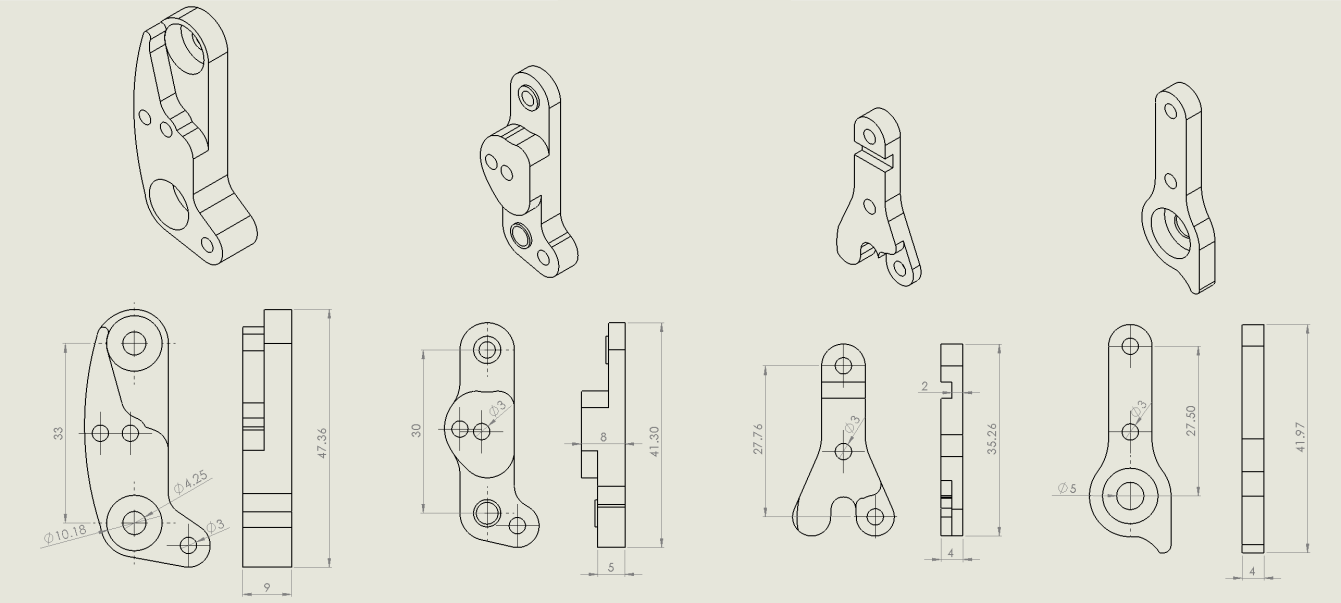
\includegraphics[width=0.9\textwidth]{Images/GripperDesign/dimensions.PNG}
    %
\includegraphics[width=0.9\textwidth]{Images/placeholder.png}
    \caption{Drawing of 4 parts and their key dimensions, 2 of each part is needed for 1 finger}
    \label{fig:dimensions}
\end{figure}

\begin{figure}
    \centering
    \begin{subfigure}{.45\linewidth}
        \centering
        %
\includegraphics[width=.4\textwidth]{Images/placeholder.png}       
        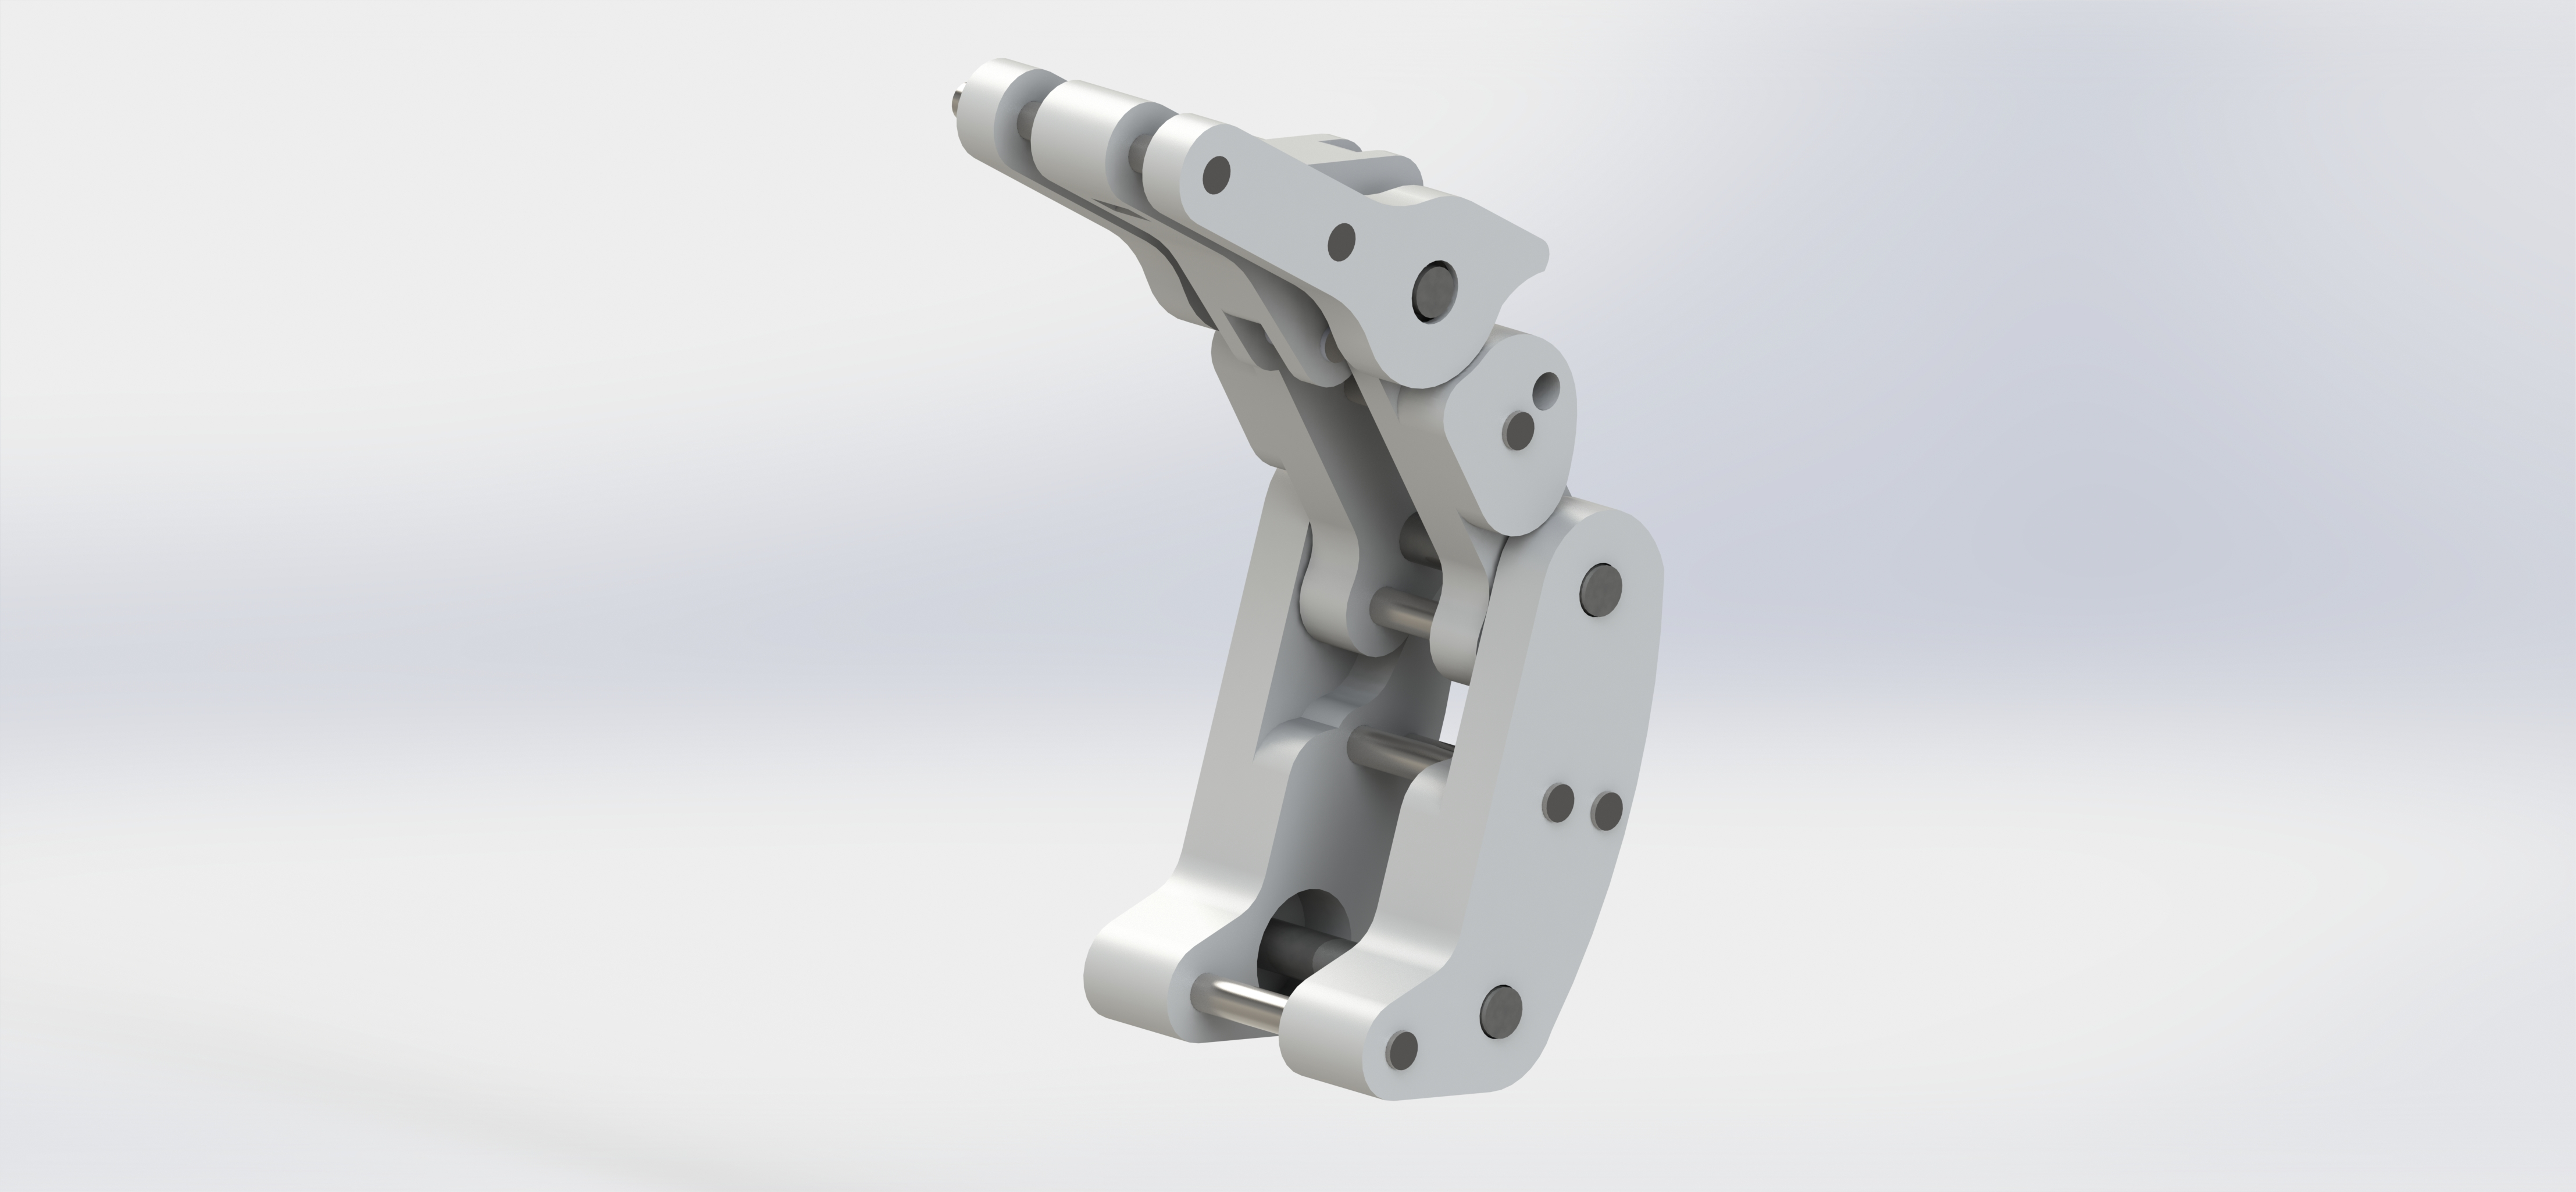
\includegraphics[width=0.9\textwidth]{Images/GripperDesign/8.JPG}
        \caption{Assembled Finger, View 1}
        \label{fig:AssFinger1}
    \end{subfigure}
    \begin{subfigure}{.45\linewidth}
        \centering
        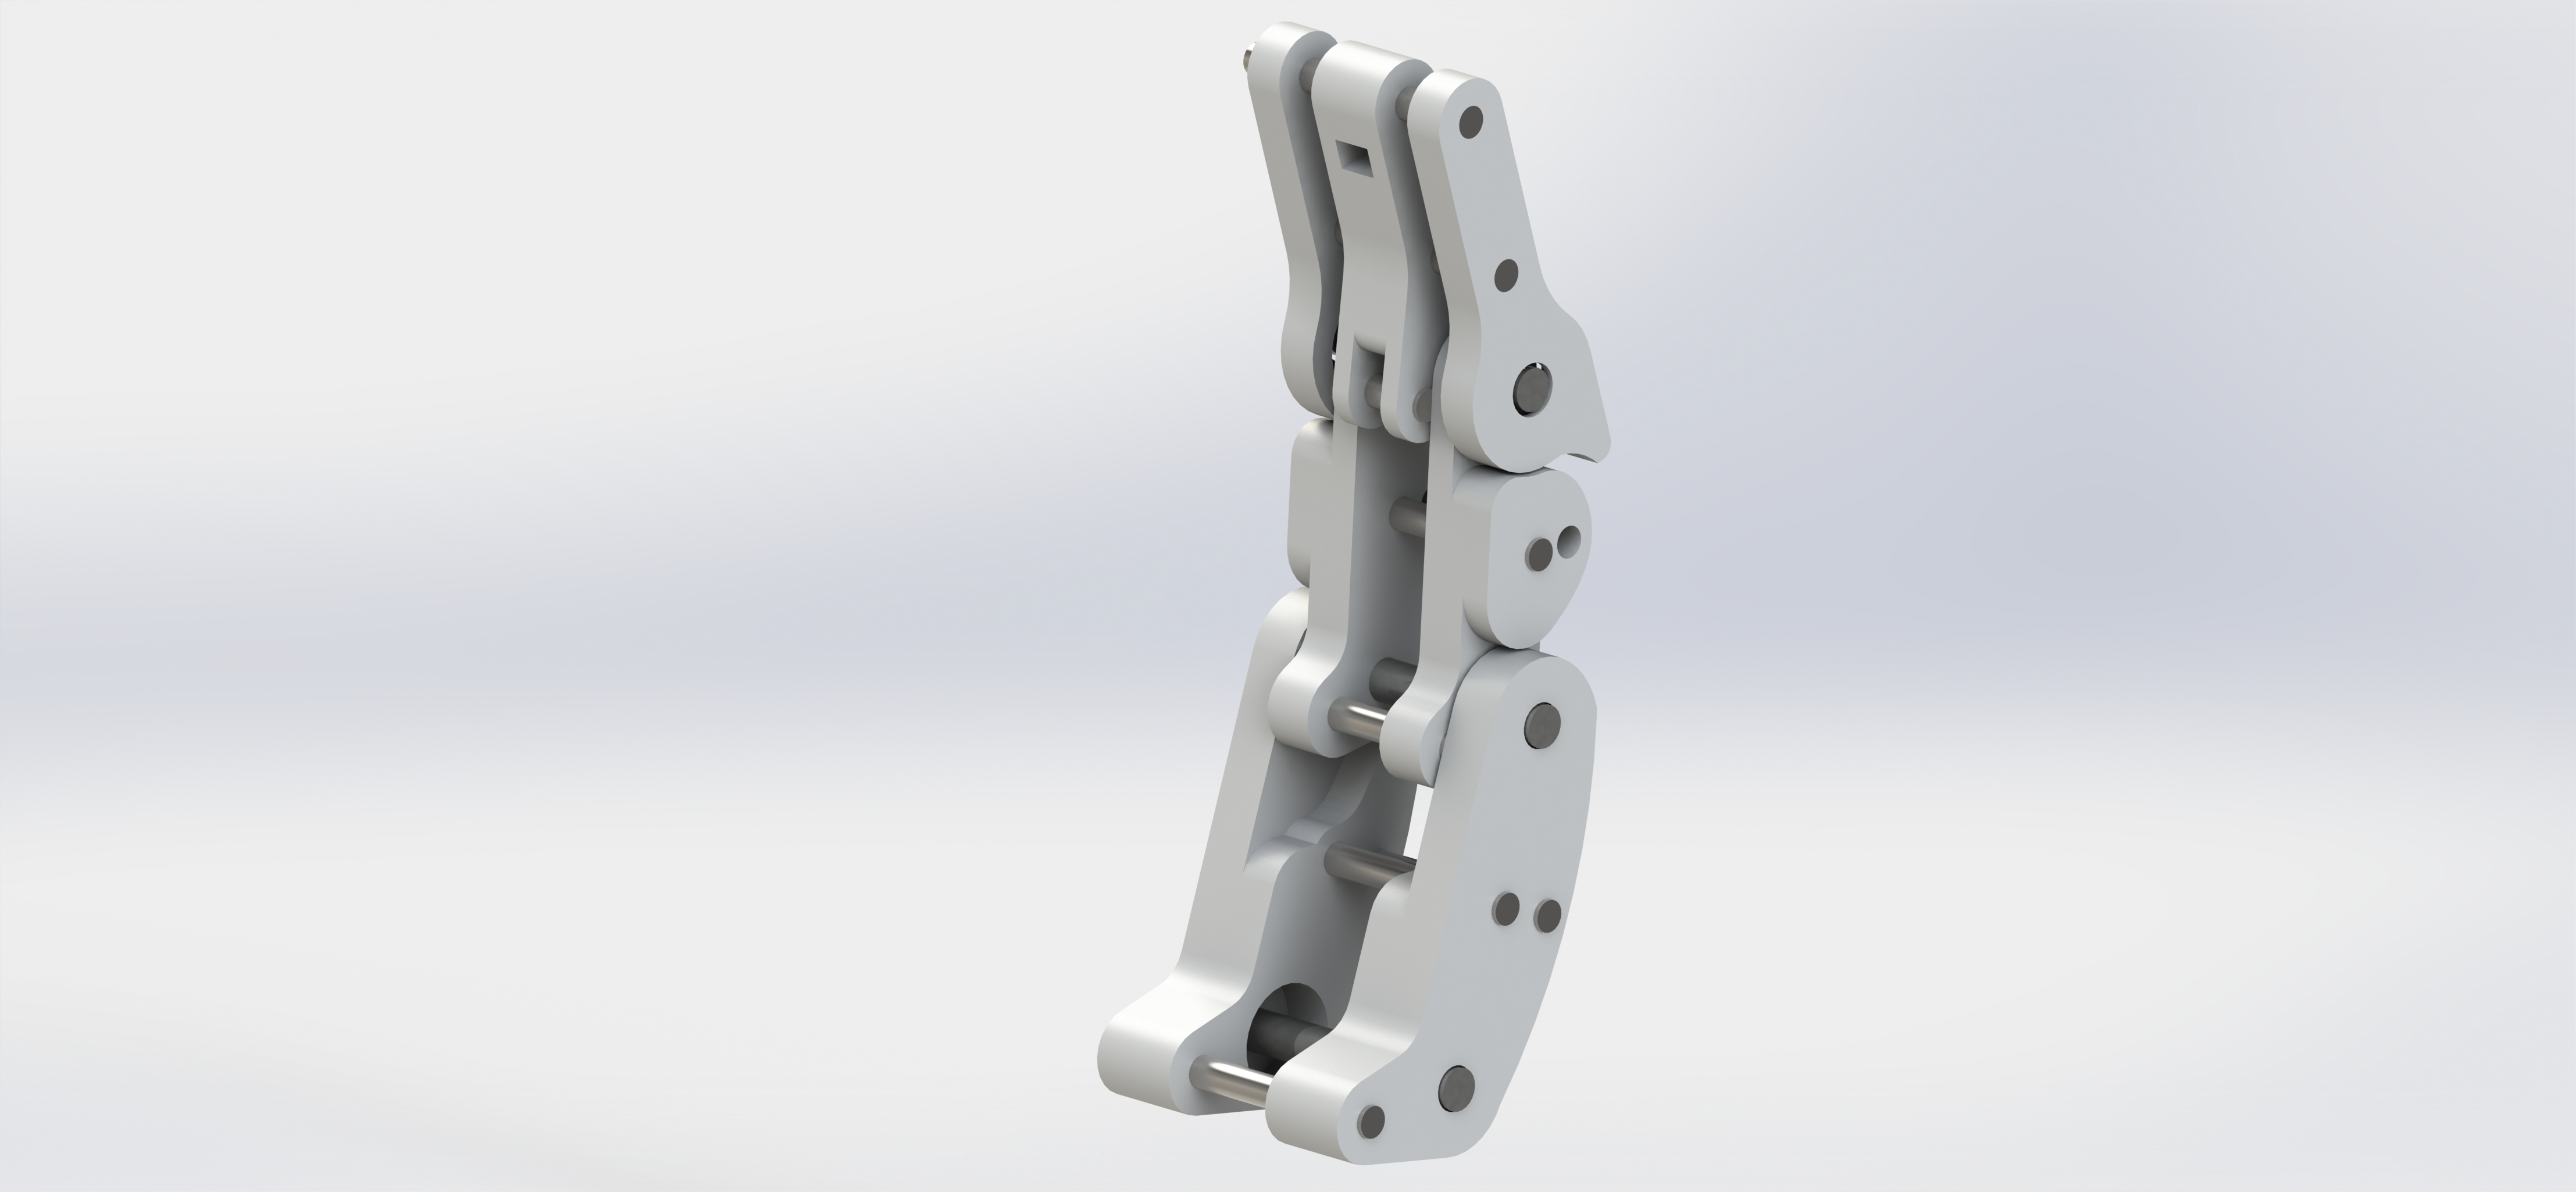
\includegraphics[width=0.9\textwidth]{Images/GripperDesign/9.JPG}
        %
\includegraphics[width=.4\textwidth]{Images/placeholder.png}
        \caption{Assembled Finger, View 2}
        \label{fig:AssFinger2}
    \end{subfigure}
    \begin{subfigure}{.45\linewidth}
        \centering
        %
\includegraphics[width=.4\textwidth]{Images/placeholder.png}       
        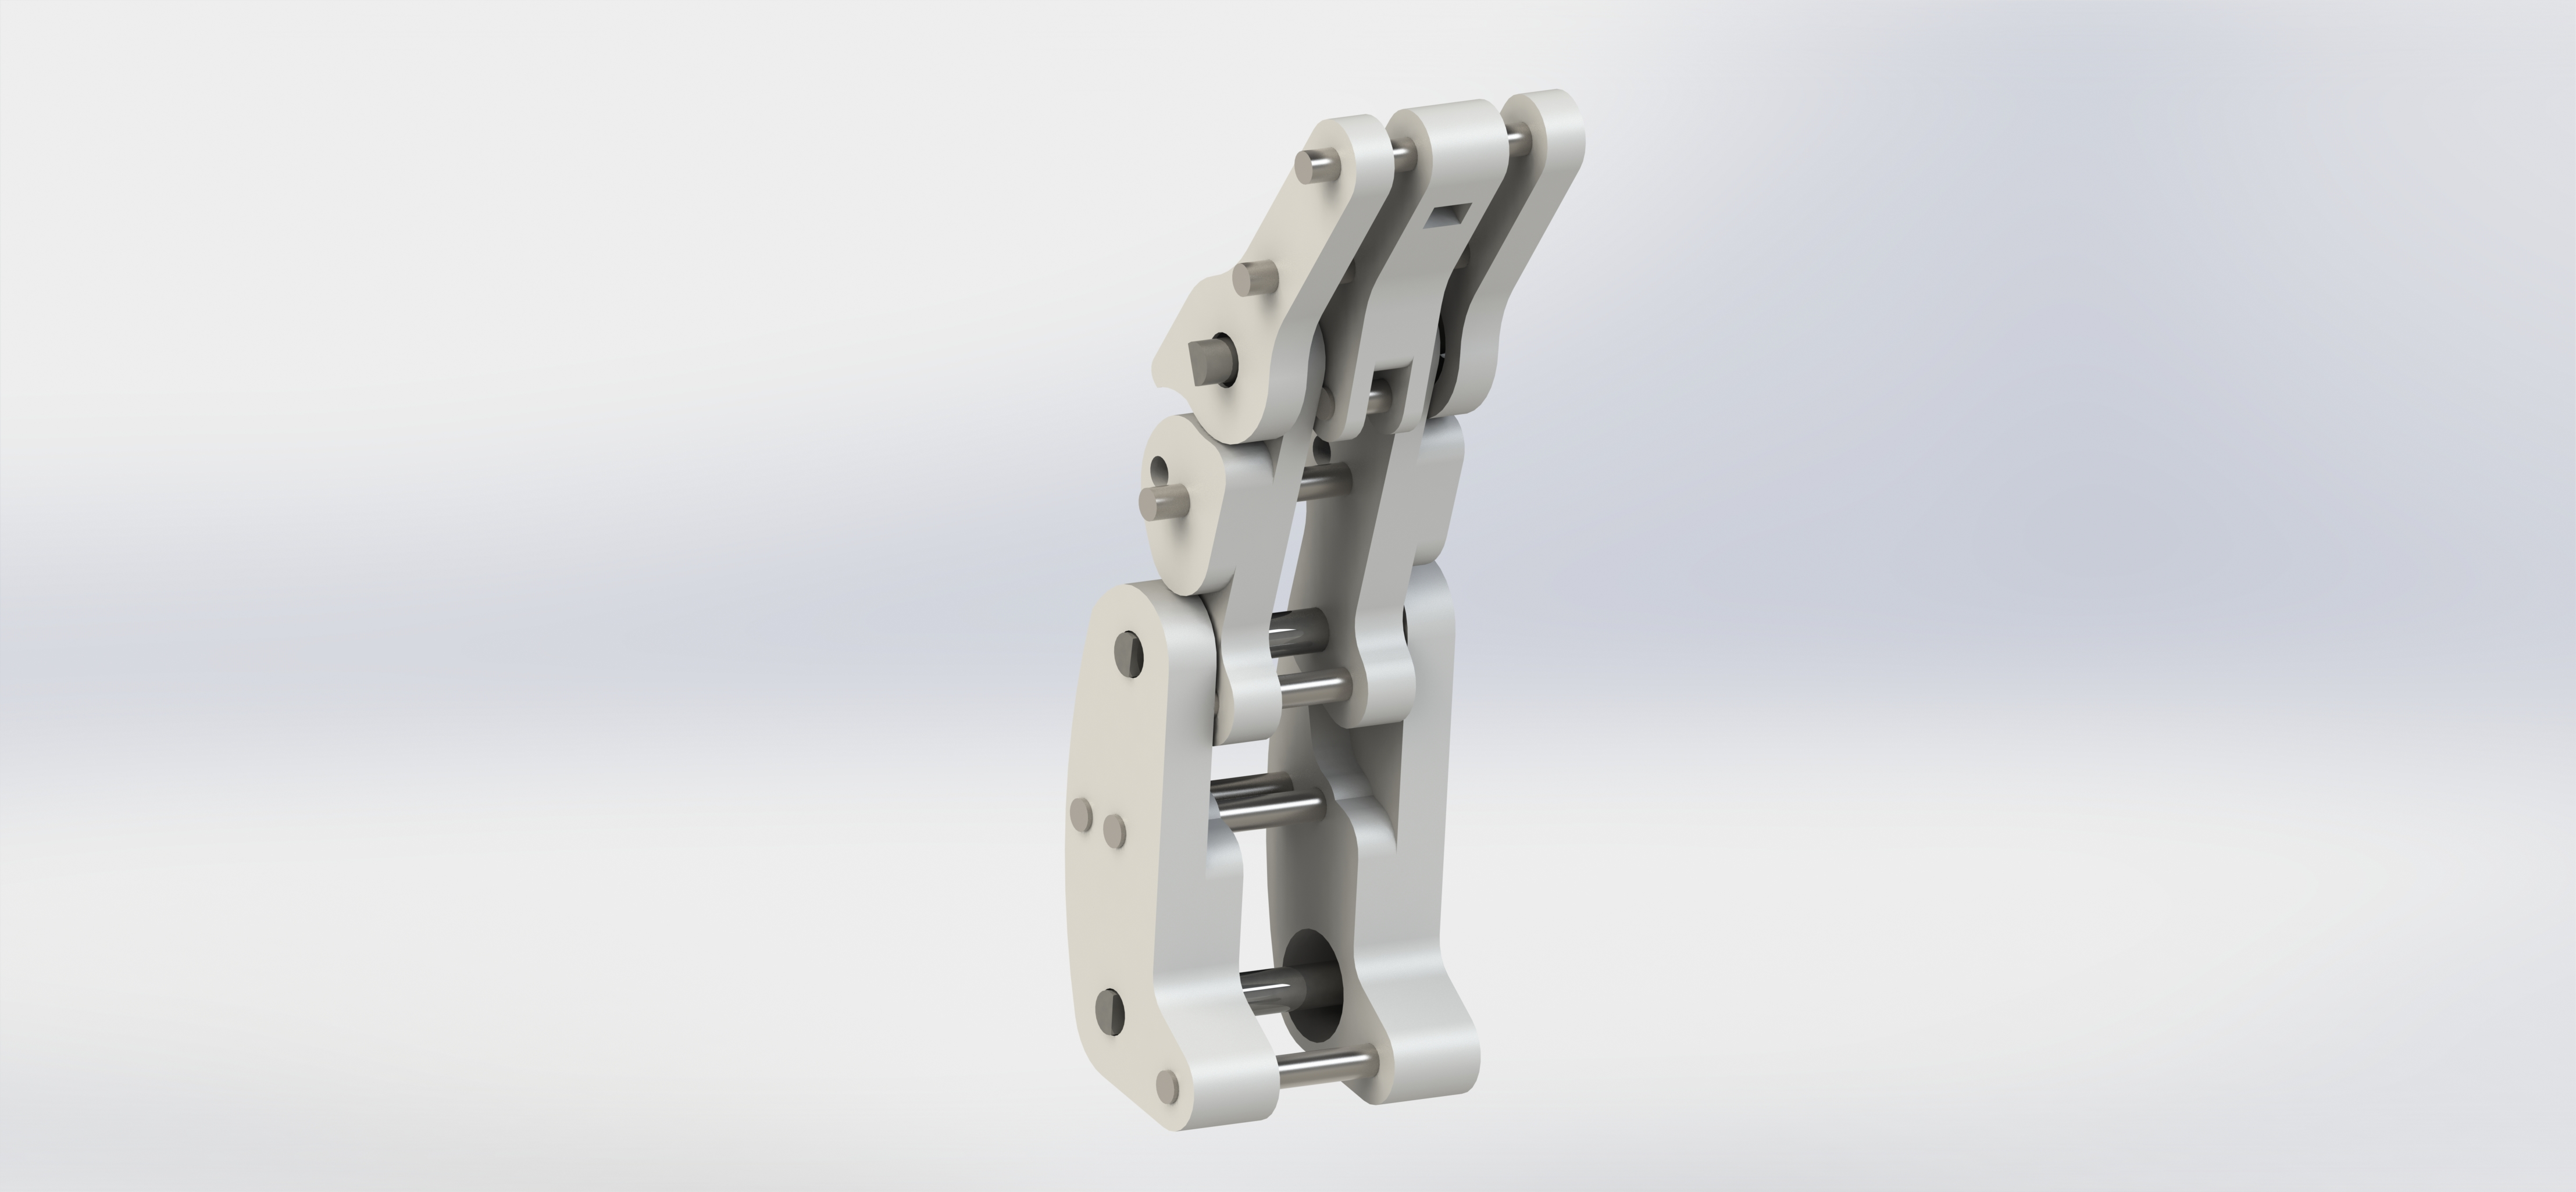
\includegraphics[width=0.9\textwidth]{Images/GripperDesign/10.JPG}
        \caption{Assembled Finger, View 3}
        \label{fig:AssFinger3}
    \end{subfigure}
    \begin{subfigure}{.45\linewidth}
        \centering
        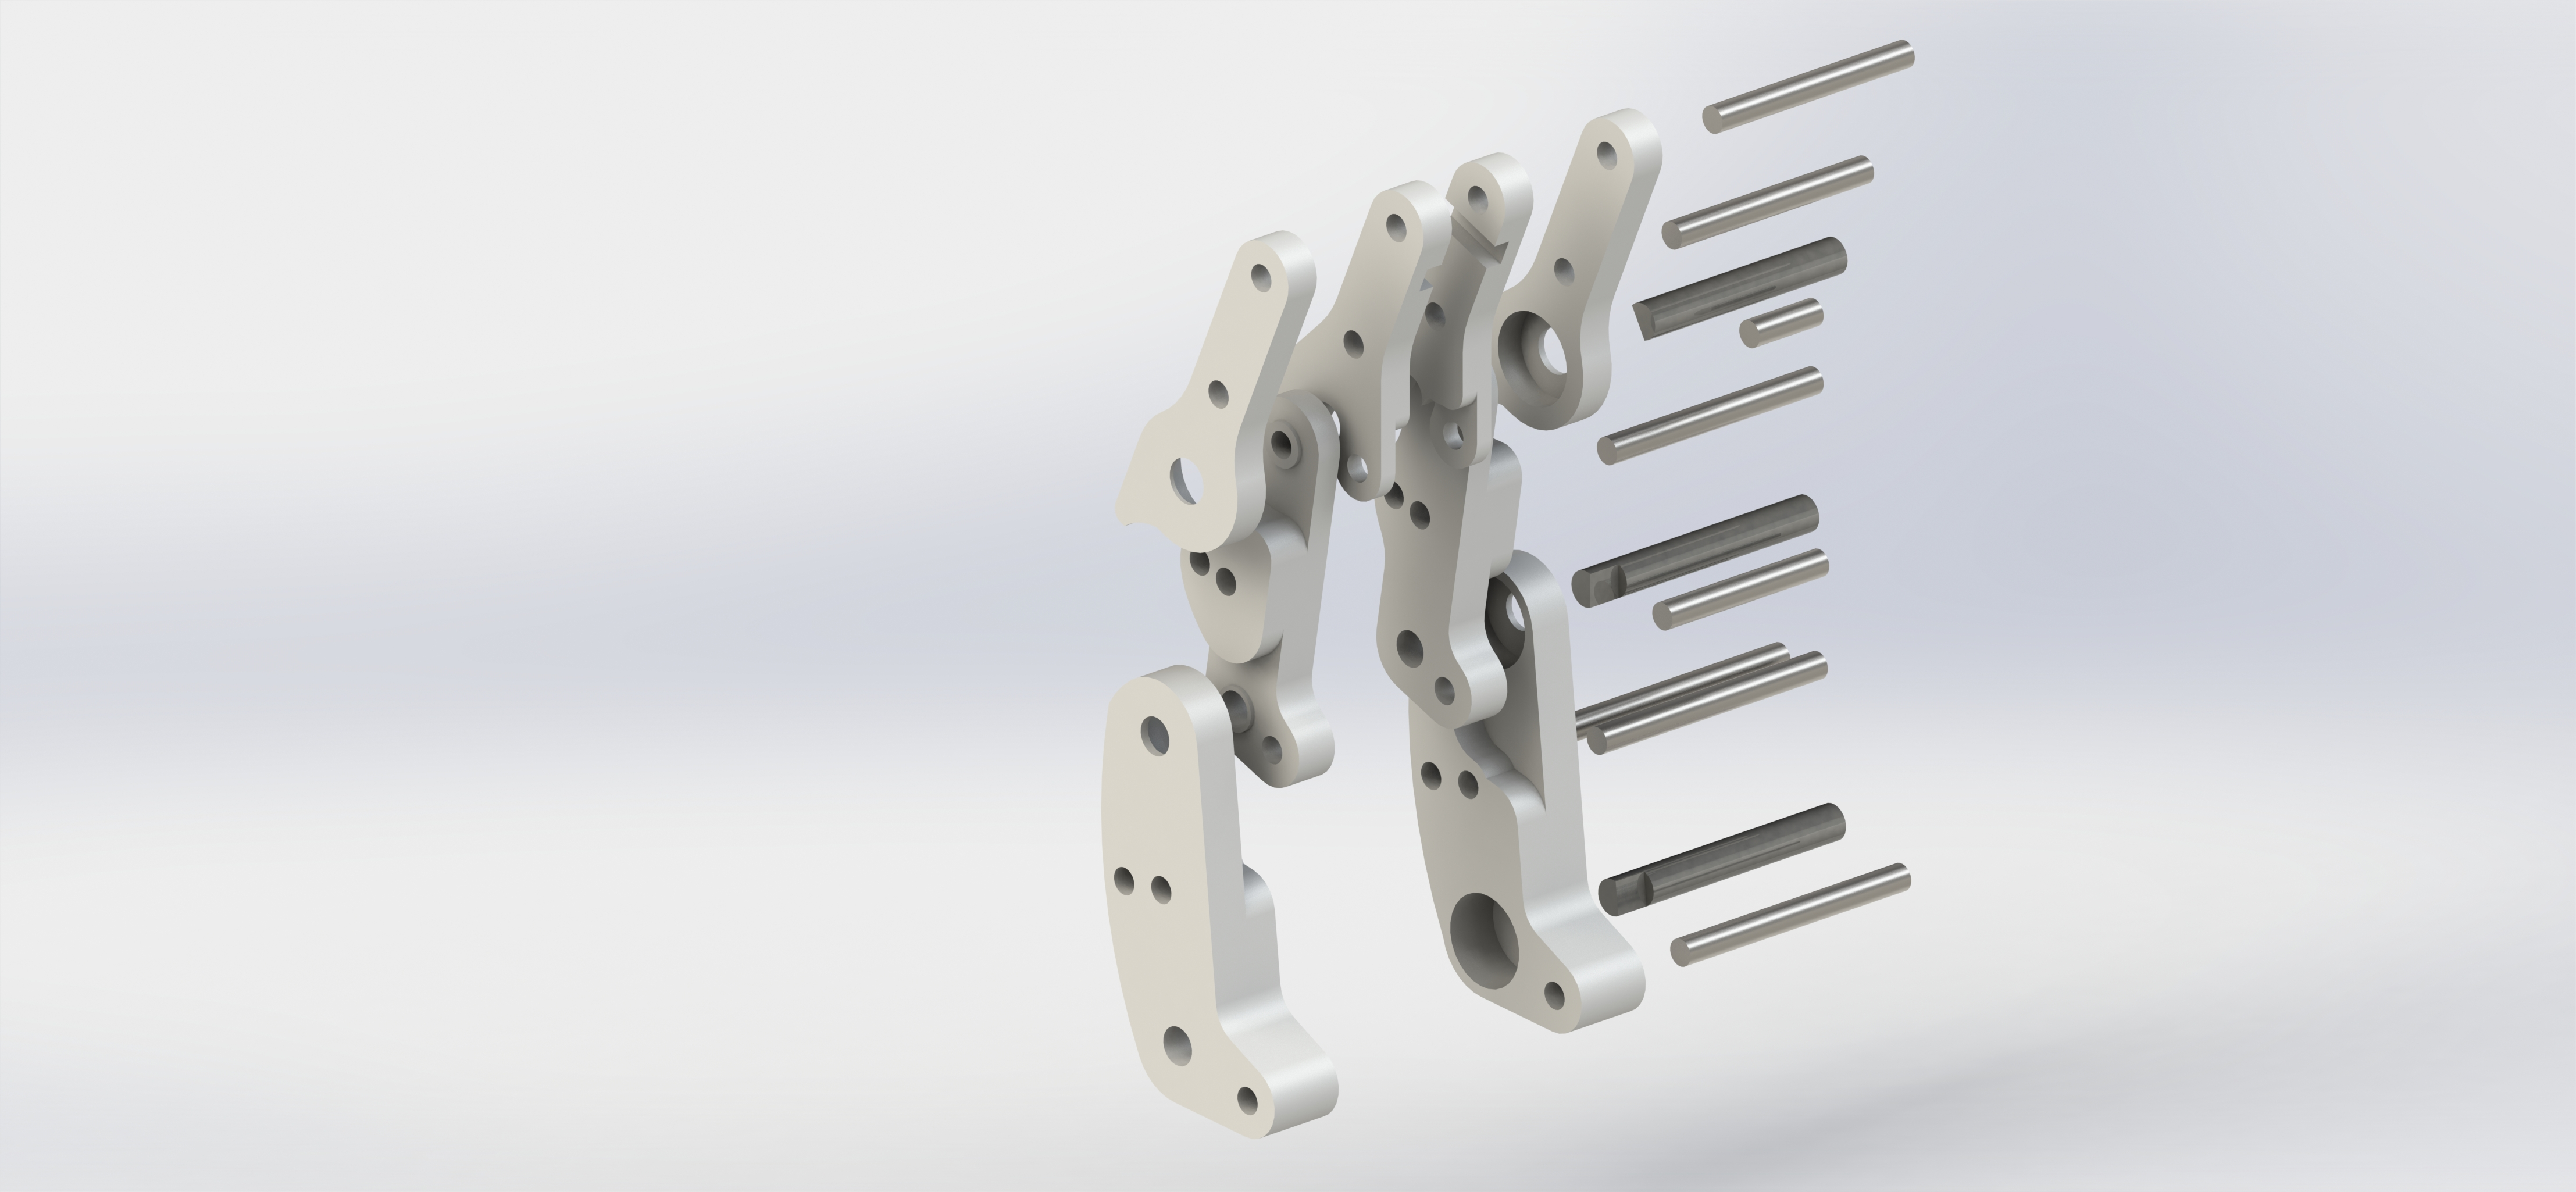
\includegraphics[width=0.9\textwidth]{Images/GripperDesign/11.JPG}          
        %
\includegraphics[width=.4\textwidth]{Images/placeholder.png} 
        \caption{Exploded View}
        \label{fig:Exploded}
    \end{subfigure}
    \begin{subfigure}{.45\linewidth}
        \centering
        %
\includegraphics[width=.4\textwidth]{Images/placeholder.png}       
        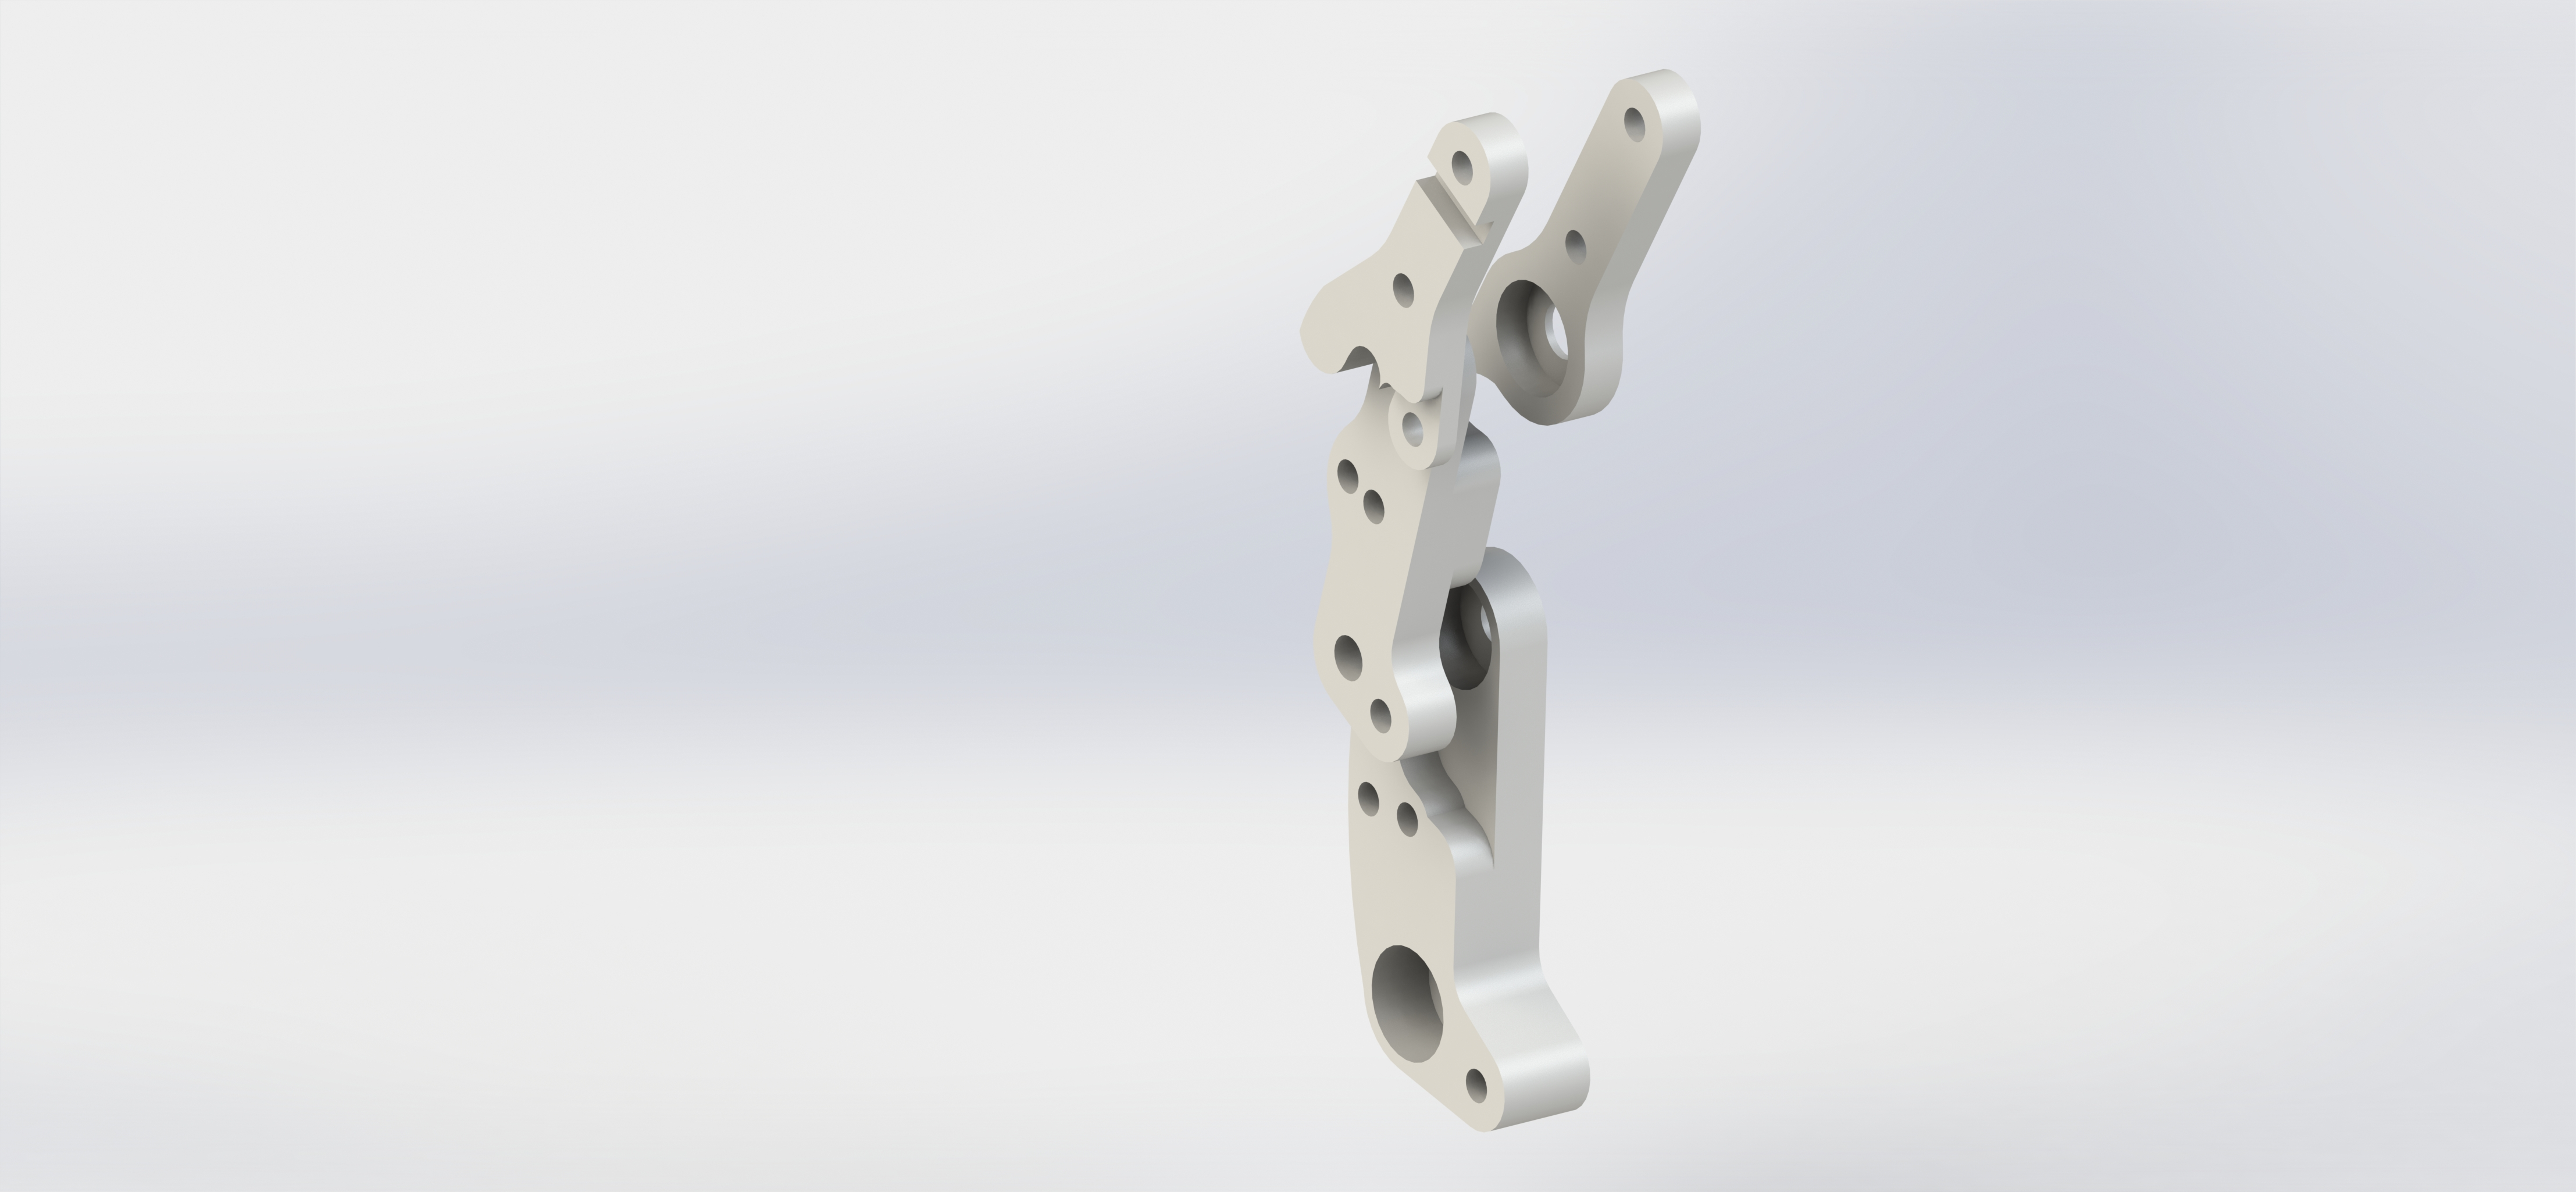
\includegraphics[width=0.9\textwidth]{Images/GripperDesign/12.JPG}
        \caption{Exploded view of 1 side of the finger}
        \label{fig:Explodedhalf}
    \end{subfigure}
    \begin{subfigure}{.45\linewidth}
        \centering
        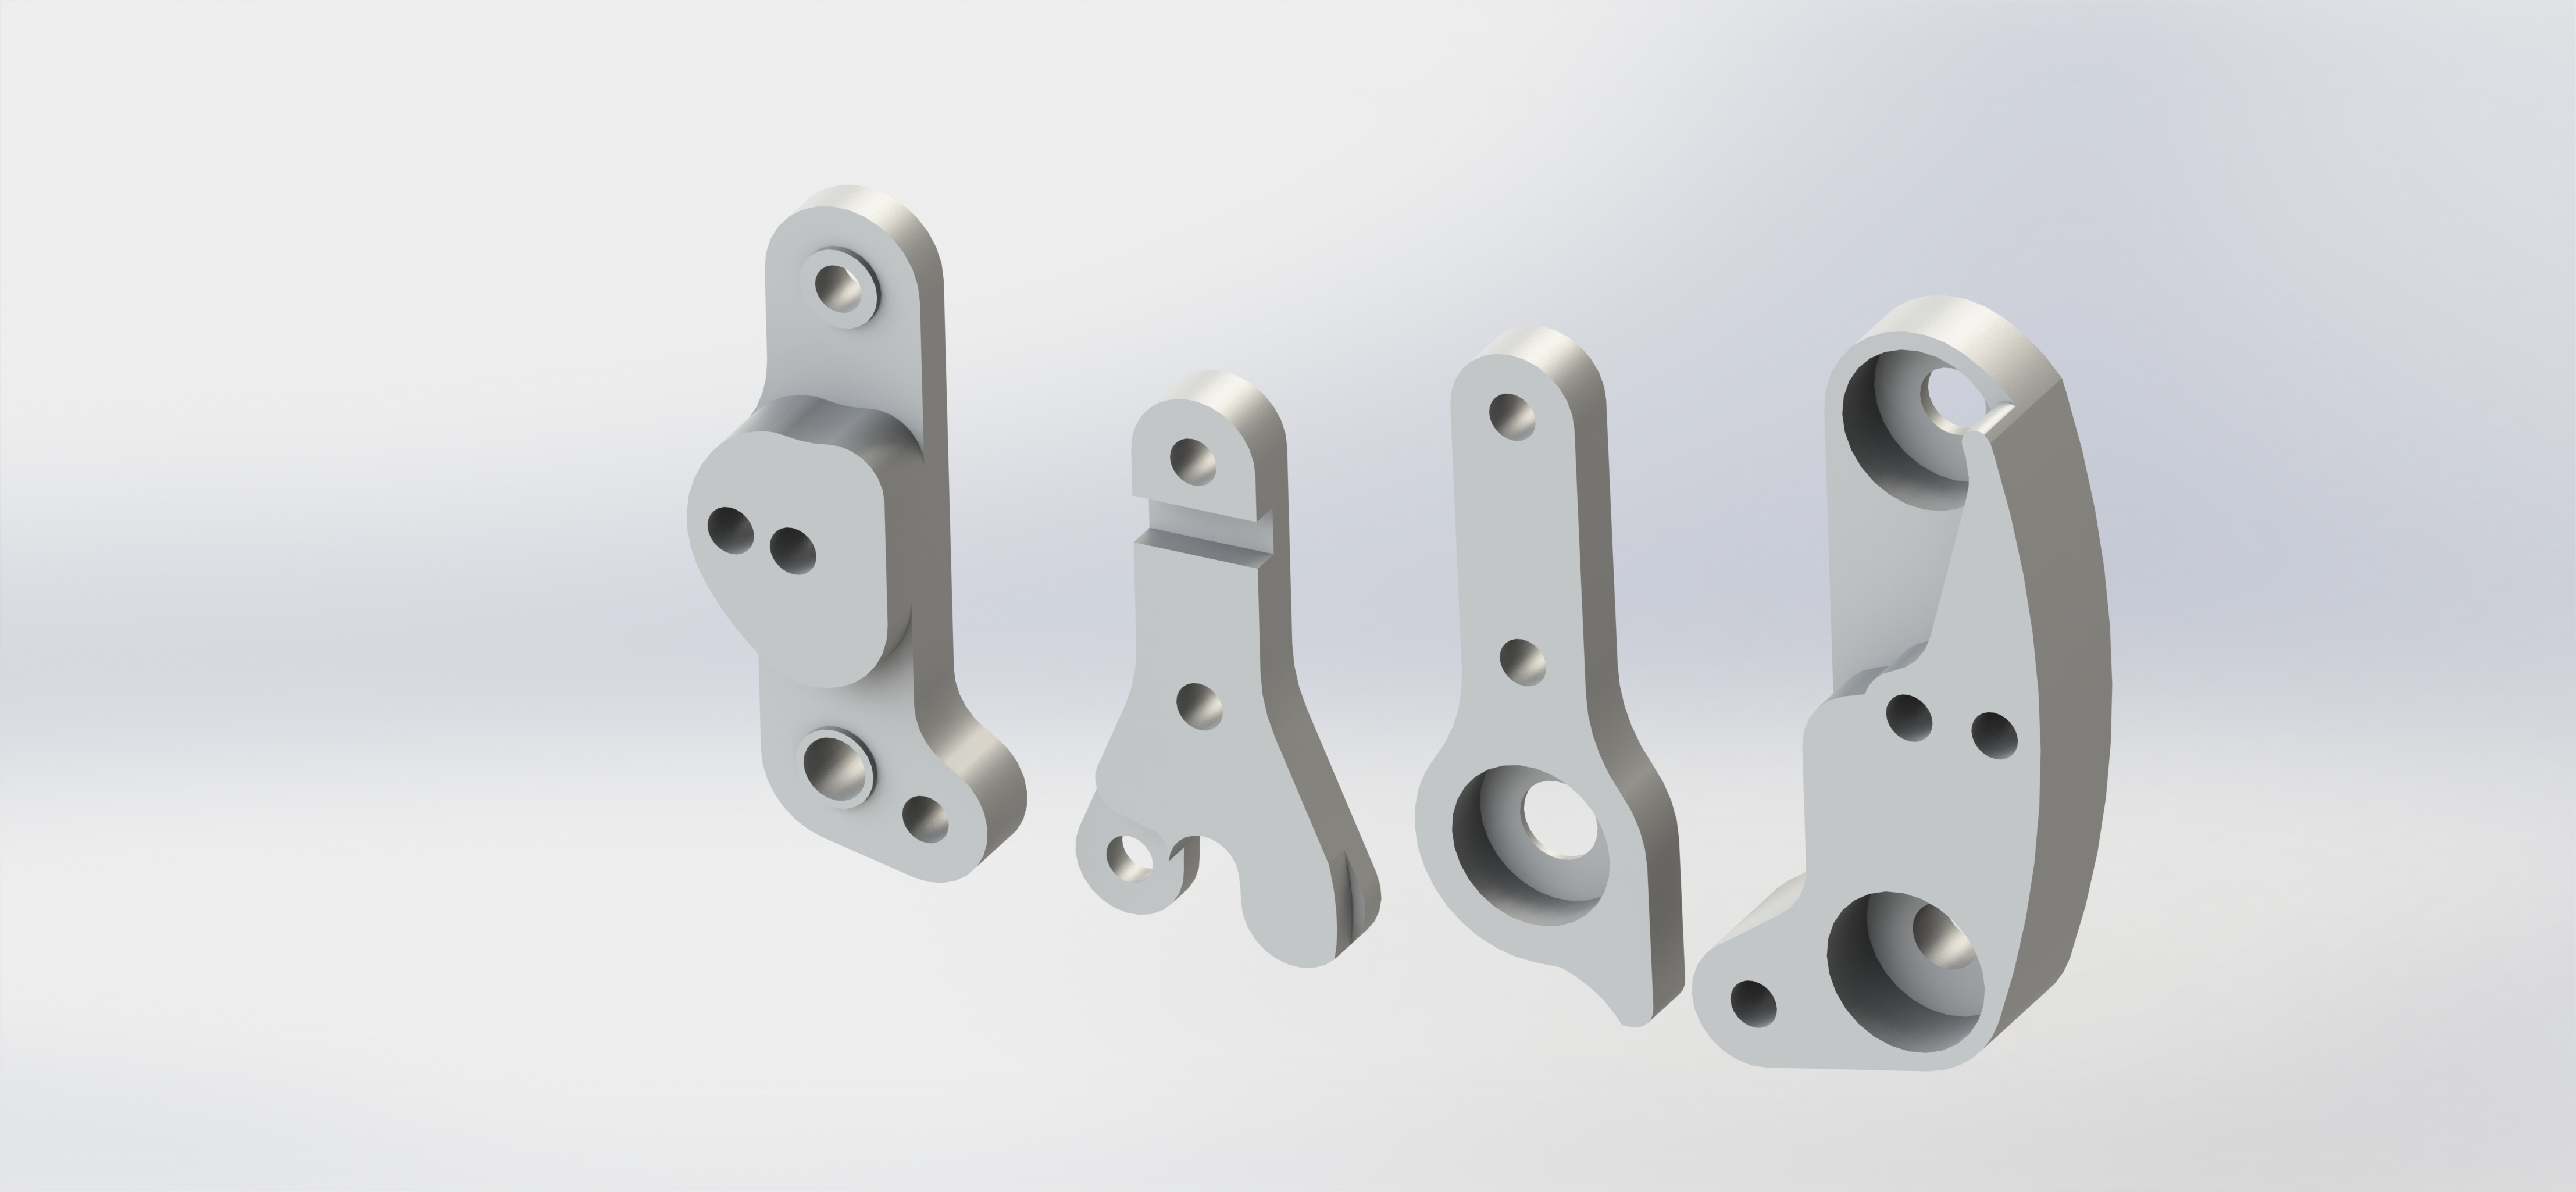
\includegraphics[width=0.9\textwidth]{Images/GripperDesign/14.JPG}          
        %
\includegraphics[width=.4\textwidth]{Images/placeholder.png} 
        \caption{4 distinct parts required}
        \label{label:}
    \end{subfigure}
    \label{fig:4Parts2}
    \caption{Parts and assemble of 1 finger}
    \label{figure:ViewsOf1Finger}
\end{figure}

\section{Actuation}
It was determined that for the purposes of the planned experiments which this gripper will be used for, that underactuation is sufficient to examine the relevant research questions. Using underactuation significantly simplifies the procedure and allows isolation of the variables under examination. As previously discussed underactuation is when the number of joints is greater than the number of actuators. When used in grasping, underactuaction gives the ability to self adapt to the object being grasped. This is achieved in this design by coupling each phalanx of the finger with an elastic element such that it will default to an open position. The design used mechanical limits to determine the relative orientation of each phalanx when open and therefore, determine the default finger position. A non-elastic element is then routed through the finger, as shown in figure \ref{figure:routing}, when actuated this will create a turning moment about each joint in turn. Starting with the bottom joint and ending with the top joint. This concept is more fully explored in Chapter \ref{LitReview} Section \ref{Actuation}\ref{UnderActuaction}

\begin{figure}
    \centering
    \begin{subfigure}{.45\linewidth}
        \centering
 %   
\includegraphics[width=.4\textwidth]{Images/placeholder.png}       
    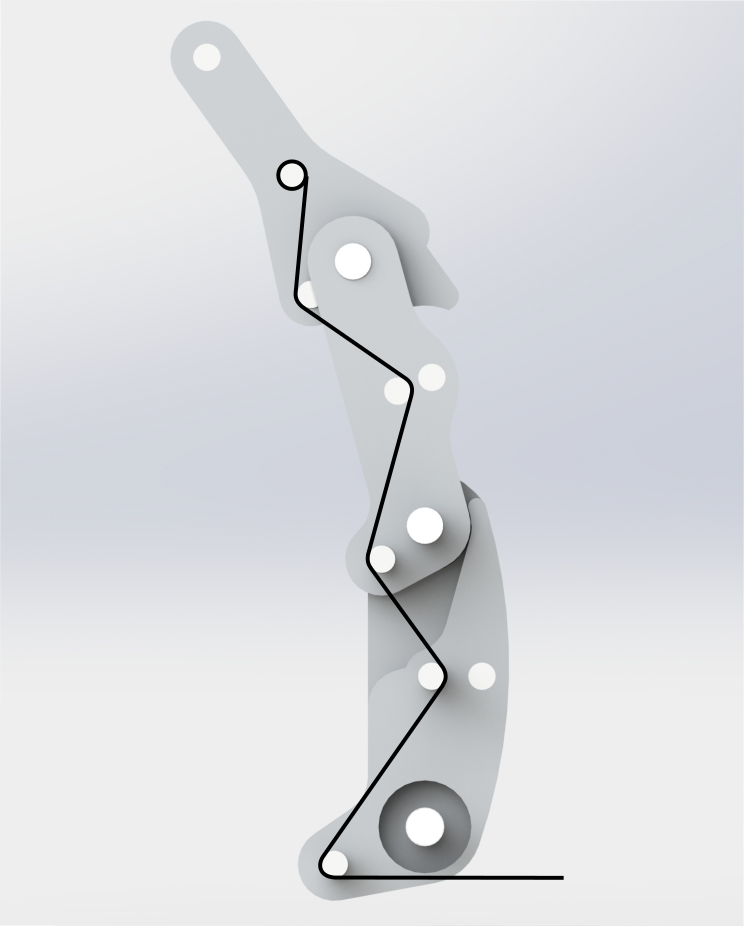
\includegraphics[width=0.7\textwidth]{Images/wirerouting/routing1.png}
        \caption{Step 1, Unactuated finger}
        \label{fig:routing1}
    \end{subfigure}
    \begin{subfigure}{.45\linewidth}
        \centering
        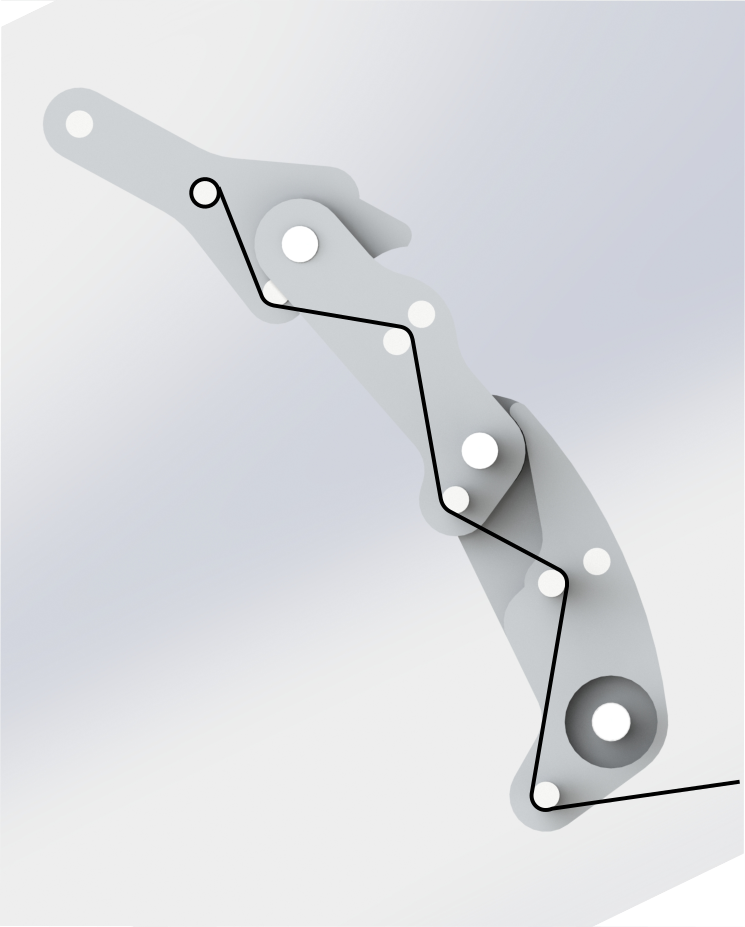
\includegraphics[width=0.7\textwidth]{Images/wirerouting/routing2.png}
%    
\includegraphics[width=.4\textwidth]{Images/placeholder.png}
        \caption{Step 2, Bottom joint begins to curl}
        \label{fig:routing2}
    \end{subfigure}
    \begin{subfigure}{.45\linewidth}
        \centering
%    
\includegraphics[width=.4\textwidth]{Images/placeholder.png}       
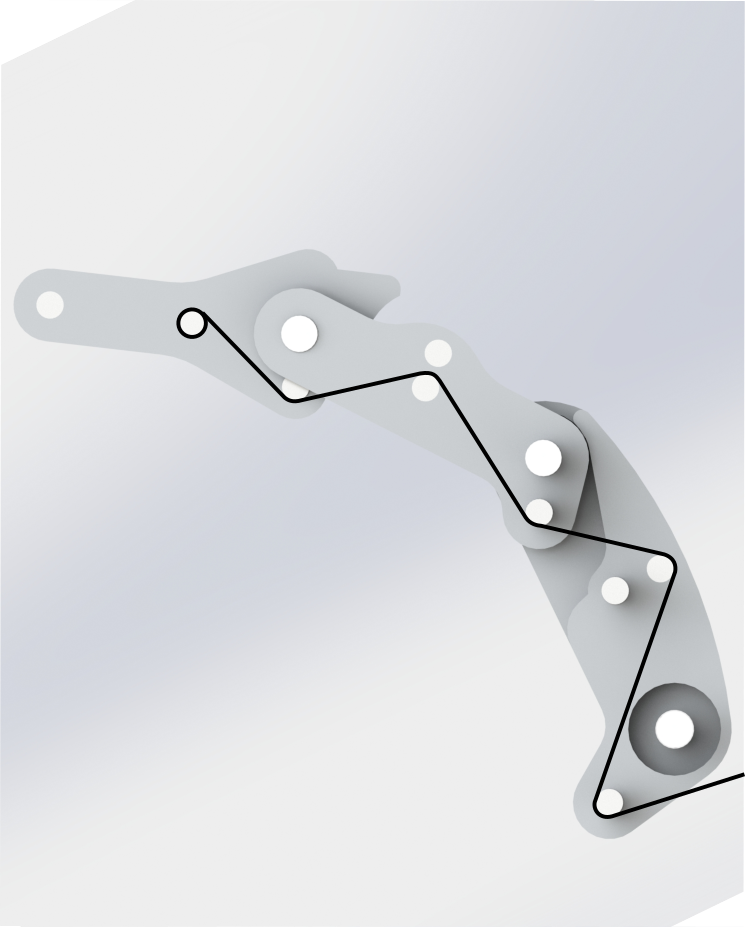
\includegraphics[width=0.7\textwidth]{Images/wirerouting/routing3.png}
        \caption{Step 3, Middle joint begins to curl}
        \label{label:routing3}
    \end{subfigure}
    \begin{subfigure}{.45\linewidth}
        \centering
        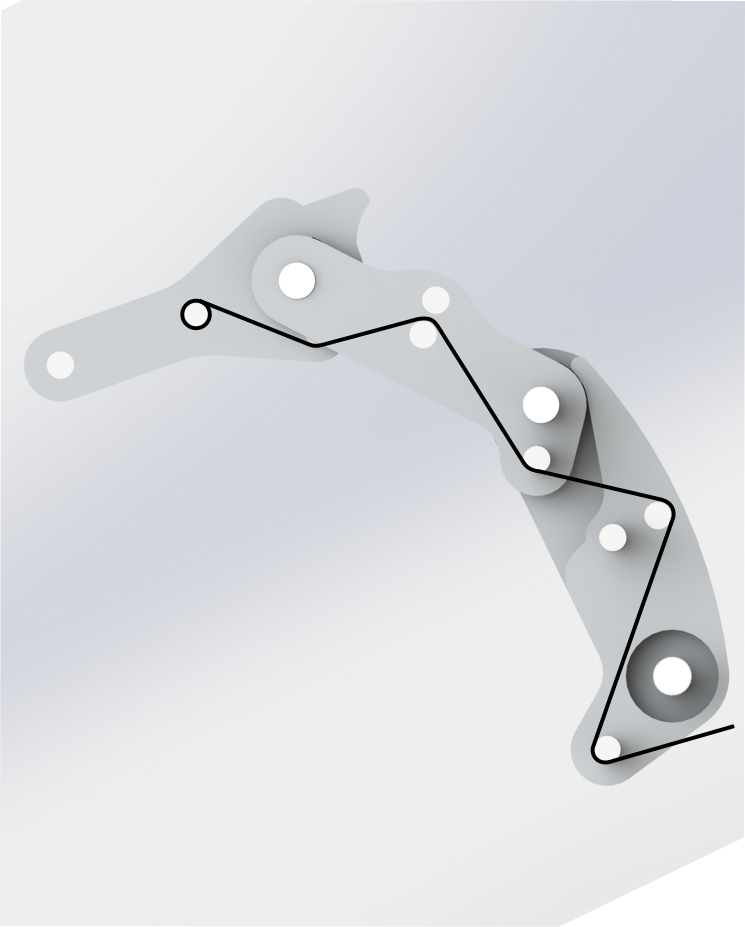
\includegraphics[width=0.7\textwidth]{Images/wirerouting/routing4.png}          
%    
\includegraphics[width=.4\textwidth]{Images/placeholder.png} 
        \caption{Step 4, Tip joint begins to curl}
        \label{label:routing4}
    \end{subfigure}
    \caption{Shows routing of wire for underactuaction}
    \label{figure:routing}
\end{figure}